\section{Optimization model and solution strategy}\label{sec:OptimizationModel}
%
This section presents the optimization problem. The rest of this section is organized as follows. First, the time sequence of decisions for participation in the mFRR market is presented. Second, we explain how scenarios for price data are generated. Third, we present the model formulation. Fourth, we discuss how the bidding policy is implemented. Lastly, we show how a scenario decomposition method with an ADMM strategy is used to solve the optimization model.

\vspace{-1mm}
\subsection{Time sequence for decision making}
Fig. \ref{fig:timeline_mfrr_variables} shows the stages for making decisions in the mFRR market. In the first stage in day $\rm{D}$-1, the BRP makes a reservation bid decision $p_{h}^{\rm{r},\uparrow}$ for every hour $h$ of day $\rm{D}$,  while being uncertain about input parameters in the next stages, including day-ahead market prices $ \lambda_{h}^{\rm{s}}$  and balancing market prices $ \lambda_{h}^{\rm{b}}$. We assume the BRP is not uncertain about mFRR market prices $ \lambda_{h}^{\rm{r}}$. 

For simplicity and avoid the need for developing a multi-stage stochastic program, we merge the second, third, and fourth stages in Fig. \ref{fig:timeline_mfrr_variables} as one, and call it the second stage. By this, $p_{h}^{\rm{r},\uparrow}$ is the first-stage variable, whereas the second stage variables, indexed by scenario $\omega$, include
the regulating power bid $\lambda_{h,\omega}^{\rm{bid}}$ and the set of real-time variables $\Gamma_{h,\omega} = \{ p_{h,\omega}, p_{h,\omega}^{\rm{b},\uparrow}$, $p_{h,\omega}^{\rm{b},\downarrow}$, $s_{h,\omega}$, $T_{h,\omega}^{\rm{c}}$, $T_{h,\omega}^{\rm{f}}$, $T_{h,\omega}^{\rm{c,\text{Base}}}$, $T_{h,\omega}^{\rm{f,\text{Base}}}$, $\phi_{h,\omega}$, $g_{h,\omega}, u^{\uparrow}_{h,\omega}, u^{\downarrow}_{h,\omega}, y^{\uparrow}_{h,\omega}, y^{\downarrow}_{h,\omega}, z^{\uparrow}_{h,\omega}, z^{\downarrow}_{h,\omega} \}$. This set contains the real-time power activated, as well as auxiliary variables for identifying up- and down-regulation,  temperature dynamics, and when to deliver up-regulation according to the bid and prices. See the Appendix for a detailed description. Note that down-regulation refers to the rebound effect of the freezer.
% \begin{figure}[!t]\label{fig:timeline_mfrr_variables}
%     \centering
%     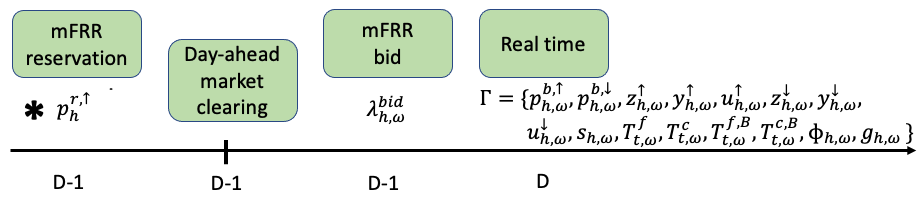
\includegraphics[width=\columnwidth]{../figures/timeline_mfrr_variables.png}
%     \caption{Variables related to mFRR up-regulation decisions. The asterisk indicates the first-stage decision.}
% \end{figure}

\begin{figure}[b]
    \centering
    \includestandalone[width=\columnwidth]{../figures/timeline_mfrr_variables_tikz}
    \caption{Variables related to the mFRR  bidding decisions.}
    \label{fig:timeline_mfrr_variables}
\end{figure}

\vspace{-1mm}
\subsection{Scenario generation}\label{sec:scenario_generation}
To make decisions on reservation capacity $p_{h}^{\rm{r},\uparrow}$ and regulating power bid $\lambda_{h,\omega}^{\rm{bid}}$, we generate a set of scenarios $\omega \in \Omega$ for spot and balancing price data., i.e., $ \lambda_{h,\omega}^{\rm{s}}$ and $ \lambda_{h,\omega}^{\rm{b}}$. Each scenario contains spot and balancing price data for the entire day in question. The number of scenarios is $|\Omega|$, and we assume all scenarios are equiprobable. We refer to them as \textit{in-sample} scenarios. We use two different strategies for in-sample scenario generation: (\textit{i}) considering historical spot and balancing prices in DK2 in 2021.
%, with different cases where the number of scenarios $|\Omega|$ is 1, 5, 10, 20, 30, 40, 50, 100, and 250. 
(\textit{ii}) considering prices of the most recent five days (lookback strategy). In both scenario generation strategies, balancing prices $\lambda_{h,\omega}^{\rm{b}}$ are sampled in the following way: First, an integer $v$ is sampled uniformly from $\{0, \ldots, 24\}$ which represents the total number of up-regulation hours in a day. We then sample spot and balancing price differentials from a single day within the set of all days where up-regulation happened $v$ times. This constitutes one scenario and is repeated $|\Omega|$ times. In this way, days where up-regulation happened are essentially up-sampled, and the model learns more when up-regulation happens than otherwise. The in-sample results are systematically compared against the same set of unseen \textit{Out-of-Sample} (OOS) scenarios, which are DK2 prices for 2022.

For load shifting, the solution approach is simply to solve a deterministic optimization problem for the next day, since the day-ahead (spot) market clearing happens in advance, and thereby the spot market prices are known.

\vspace{-1mm}
\subsection{Model formulation}
Recall that \eqref{eq:mFRRObjective} gives the objective function of a BRP participating in the mFRR market, but in a deterministic setup.  The optimization problem of such a BRP in a two-stage stochastic programming format is
%
\begin{subequations}\label{P1:compact_model}
    \begin{align}
        \underset{\bm{p}^{\rm{r},\uparrow}, \bm{\lambda}_{\omega}^{\rm{bid}}, \bm{\Gamma}_{\omega}}{\text{Maximize}} \ & f(\bm{p}^{\rm{r},\uparrow}) + \sum_{\omega \in \Omega} \pi_{\omega} \ g(\bm{\Gamma}_{\omega}) \label{P1:eq1}
        \\
        \text{s.t.} \                                                                                            & h(\bm{p}^{\rm{r},\uparrow}, \bm{\lambda}_{\omega}^{\rm{bid}}, \bm{\Gamma}_{\omega}) \leq 0, \ \forall{\omega}\label{P1:eq2}                                                                                             \\
        \                                                                                                        & \text{State-space model } (\ref{eq:2ndFreezerStateSpace}), \ \forall{\omega} \label{P1:eq3}
        \\
        \                                                                                                        & \bm{T}_{\omega}^{\rm{c}}, \bm{T}_{\omega}^{\rm{f}},  \bm{T}_{\omega}^{\rm{c,\text{Base}}}, \bm{T}_{\omega}^{\rm{f,\text{Base}}}\in \mathbb{R}  \label{P1:eq4}
        \\
                \                                                                                                        & \bm{p}_{\omega}, \bm{p}^{\rm{r},\uparrow}, \bm{\lambda}_{\omega}^{\rm{bid}}, \bm{p}_{\omega}^{\rm{b},\uparrow}, \bm{p}_{\omega}^{\rm{b},\downarrow}, \bm{s}_{\omega},  \bm{\phi}_{\omega}\in \mathbb{R}^{+}  \label{P1:eq5}
        \\
        \                                                                                                        & \bm{g}_{\omega}, \bm{u}^{\uparrow}_{\omega}, \bm{z}^{\uparrow}_{\omega}, \bm{y}^{\uparrow}_{\omega}, \bm{u}^{\downarrow}_{\omega}, \bm{z}^{\downarrow}_{\omega}, \bm{y}^{\downarrow}_{\omega} \in \{0,1\},  \label{P1:eq6}
    \end{align}
\end{subequations}
%
where bold symbols represent vectors. For example, the vector $\bm{p}^{\rm{r},\uparrow}$ includes $p_{h}^{\rm{r},\uparrow} \ \forall{h}$. Parameter $\pi_{\omega}$ is the probability assigned to in-sample scenario $\omega$. Here, we present optimization \eqref{P1:compact_model} in a compact form using functions $f(.)$, $g(.)$, and $h(.)$. The detailed formulation is given in the Appendix. Constraint (\ref{P1:eq2}) includes all power and activation related limits, whereas (\ref{P1:eq3}) models temperature dynamics in the freezer. Constraints (\ref{P1:eq4})-(\ref{P1:eq5}) declare continuous and binary variables. Note that $\mathbb{R}$ and $\mathbb{R}^{+}$ denote free and non-negative real numbers, respectively. The optimization model \eqref{P1:compact_model} is a MILP problem.


For optimal decision making for load shifting, \eqref{P1:compact_model} is simplified by removing scenarios as well as reservation and bid constraints, and replacing the objective function (\ref{P1:eq1}) by minimizing the total power purchase cost $\bm{\lambda}^{\rm{s}} \bm{p}$.

\vspace{-1mm}
\subsection{Regulating power bidding implementation}\label{sec:mFRR_bidding_implementation}
Recall from  Fig. \ref{fig:timeline_mfrr_variables} that we have merged three stages, by which the regulating power bidding decisions $\lambda_{h,\omega}^{\rm{bid}}$ and real-time operational decisions $\Gamma_{h,\omega}$ become second-stage variables. This is the reason both set of variables $\lambda_{h,\omega}^{\rm{bid}}$ and $\Gamma_{h,\omega}$ are similarly indexed by $\omega$, while in reality, the decision $\lambda_{h,\omega}^{\rm{bid}}$ should be made before $\Gamma_{h,\omega}$. This also challenges the ex-post OOS simulation. To resolve it, we use a learning policy, such that we replace the scenario-indexed variable $\lambda_{h,\omega}^{\rm{bid}}$ in \eqref{P1:compact_model} by $\alpha q(\lambda_{h,\omega}^{\rm{s}}) + \beta$, where $q(.)$ is an arbitrarily selected function. In addition, $\alpha$ and $\beta$ are non-negative first-stage  variables (they are not indexed by $\omega$). This replacement shrinks the degree of freedom for the BRP compared to \eqref{P1:compact_model}, but makes it more practical to be used. The reason is that, by this trick, the regulating power bidding decision to be made at 5pm of day $\rm{D}$-1 becomes a first-stage decision, dependent not only on policies $\alpha$ and $\beta$, but also on uncertain spot prices $\lambda_{h,\omega}^{\rm{s}}$. In other words, by using the in-sample scenarios $\omega$, the BRP obtains optimal values for $\alpha$ and $\beta$ at 9:30am of day $\rm{D}$-1. Then, she waits to see the spot prices at noon of day $\rm{D}$-1, and  submits her regulating power bids at 5pm of day $\rm{D}$-1. In our simulations, we found out that the selection of $q(\lambda_{h,\omega}^{\rm{s}})$ as the difference of spot prices in subsequent hours works comparatively more satisfactory ex-post, as it suits better to accommodate the rebound effect. By this, the BRP prefers to be activated when the spot price during rebound (down-regulation) is comparatively lower. Therefore, we replace $\lambda_{h,\omega}^{\rm{bid}}$ in \eqref{P1:compact_model} by
%
\begin{align}\label{eq:affine_policy}
     & \alpha ( \lambda_{h+1,\omega}^{\rm{s}} - \lambda_{h,\omega}^{\rm{s}}) + \lambda_{h,\omega}^{\rm{s}} + \beta, \ \forall{\omega}, \forall{h} \in \{1, \ldots, 23\}.
\end{align}



%To solve Problem (\ref{P1:compact_model}), we first need to specify a bidding policy that can readily be used OOS. We do so by choosing an affine bidding policy. Afterwards, it is shown how the bidding policy is implemented using McCormick relaxation.

%\subsubsection{Affine bidding policy}

%A bidding policy needs to be easy to follow OOS for the trader. We choose an affine bidding policy, i.e., a linear function of the spot price. The bidding policy is given by:





%Variables $\alpha$ and $\beta$ are then learned IS and fixed for OOS evaluation. After the day-ahead market clearing, (\ref{eq:affine_policy}) can easily be used to specify bids for the next day.

Another implementation challenge is to enforce price conditions under which the mFRR reservation is activated.
Recall from Section \ref{sec:mFRR}, for the activation at hour $h$ under scenario $\omega$, it is necessary to hold $\lambda_{h,\omega}^{\rm{bid}} \leq  \lambda_{h,\omega}^{\rm{b}} - \lambda_{h,\omega}^{\rm{s}}$ and $ \lambda_{h,\omega}^{\rm{b}} > \lambda_{h,\omega}^{\rm{s}}$. These conditions can be equivalently enforced as
%
%activation of mFRR reservation only happens when certain price conditions are met. This is formalized in the following constraint:
%
\begin{equation}\label{eq:bid_constraint}
    p^{\rm{b}, \uparrow}_{h,\omega} + s_{h,\omega} \geq p^{\rm{r},\uparrow}_{h}  \mathbbm{1}^{\big(\lambda_{h,\omega}^{\rm{bid}} \leq  \lambda_{h,\omega}^{\rm{b}} - \lambda_{h,\omega}^{\rm{s}} \ \text{and} \ \lambda^{\rm{b}}_{h,\omega} > \lambda^{\rm{s}}_{h,\omega}\big)},
\end{equation}
where $\mathbbm{1}^{(.)}$ is 1 if conditions (.) are met, otherwise it is zero. If the non-negative slack variable $s_{h,\omega}$ takes a non-zero value, it shows that the BRP fails in the activation stage, and therefore will be penalized. The challenge is that \eqref{eq:bid_constraint} makes a condition on variable $\lambda_{h,\omega}^{\rm{bid}}$, or equivalently on $\alpha$ and $\beta$ as defined in \eqref{eq:affine_policy}. This makes \eqref{eq:bid_constraint} non-linear. To linearize it, we use the McCormick relaxation technique \cite{mccormick1976computability} and define auxiliary  variables $\phi_{h,\omega} \in \mathbb{R}^{+}$ and $g_{h,\omega} \in \{0, 1\}$. By this, we replace \eqref{eq:bid_constraint} for every hour $h$ and scenario $\omega$ by a set of mixed-integer linear constraints as
%
%Eq. (\ref{eq:bid_constraint}) shows how real-time up-regulation plus a slack variable must be greater than or equal to the reservation if the bid is lower than the balancing price and if up-regulation is needed in hour $h$. It is a bi-linear constraint so McCormick relaxation \cite{mccormick1976computability} is used to convert (\ref{eq:bid_constraint}) to a linear constraint by introducing auxiliary variables, $\phi_{h,\omega}$ and $g_{h,\omega}$:
%
\begin{subequations}\label{eq:bid_constraint_relaxed}
    \begin{align}
       & \lambda_{h,\omega}^{\rm{bid}} - M  (1 - g_{h,\omega}) \leq \lambda_{h,\omega}^{\rm{b}} - \lambda_{h,\omega}^{\rm{s}} \leq \lambda_{h,\omega}^{\rm{bid}} + M  g_{h,\omega},                               \label{con_bid:subeq1}\\
        & p^{\rm{b}, \uparrow}_{h,\omega} \leq \phi_{h,\omega}  \mathbbm{1}^{\lambda^{\rm{b}}_{h,\omega} > \lambda^{\rm{s}}_{h,\omega}}, \                          \label{con_bid:subeq3}  \\
        &p^{\rm{b}, \uparrow}_{h,\omega} + s_{h,\omega} \geq \phi_{h,\omega}  \mathbbm{1}^{\lambda^{\rm{b}}_{h,\omega} > \lambda^{\rm{s}}_{h,\omega}}, \            \label{con_bid:subeq4}  \\
        &-g_{h,\omega}  M \leq \phi_{h,\omega} \leq g_{h,\omega}  M,                                   \label{con_bid:subeq5}  \\
        &-(1 - g_{h,\omega})  M \leq \phi_{h,\omega} - p^{\rm{r},\uparrow}_{h} \leq (1 - g_{h,\omega}) M, \                                                                                    \label{con_bid:subeq7}  \
        % \lambda_{h,\omega}^{\rm{bid}} \leq \lambda^{Max} \label{con_bid:subeq9}
    \end{align}
\end{subequations}
where $M$ is a large enough positive constant.
Constraint \eqref{con_bid:subeq1} ensures that $g_{h,\omega} = 1$ when $\lambda_{h,\omega}^{\rm{b}} - \lambda_{h,\omega}^{\rm{s}} \geq \lambda^{\rm{bid}}_{h, \omega}$. Otherwise, it sets $g_{h,\omega} = 0$. Constraints \eqref{con_bid:subeq3}-\eqref{con_bid:subeq4} set the up-regulation equal to $\phi_{h,\omega}$ (or incurs a penalty through $s_{h,\omega}$) if there is an up-regulation event in the system, i.e., if $\mathbbm{1}^{\lambda^{\rm{b}}_{h,\omega} > \lambda^{\rm{s}}_{h,\omega}} = 1$. Constraint \eqref{con_bid:subeq5} enforces  $\phi_{h,\omega} = 0$ when $g_{h,\omega} = 0$, implying the balancing price minus the spot price is smaller than the power regulating bid. Constraint \eqref{con_bid:subeq7} ensures that $\phi_{h,\omega}$ is equal to the reservation capacity $p^{\rm{r},\uparrow}_{h}$ whenever $g_{h,\omega} = 1$, i.e., if $\lambda_{h,\omega}^{\rm{b}} - \lambda_{h,\omega}^{\rm{s}} \geq \lambda^{\rm{bid}}_{h, \omega}$. Note that in the final model,  $\lambda^{\rm{bid}}_{h, \omega}$ in \eqref{eq:bid_constraint_relaxed} should be replaced as defined in \eqref{eq:affine_policy}. The resulting model formulation, which is a MILP, is given in the Appendix.

\vspace{-1mm}
\subsection{Scenario decomposition with ADMM}
By increasing the number of scenarios,  the proposed stochastic program  quickly becomes computationally intractable due to the number of binary variables and intertemporal constraints. To resolve it, we apply a scenario decomposition approach built upon the ADMM algorithm \cite{boyd2011distributed}. To do so, we relax non-anticipativity constraints by adding a scenario index to the first-stage variables, i.e.,
%
\begin{equation}\label{eq:non_anticipativity}
    p_{h}^{\rm{r},\uparrow} \rightarrow p^{\rm{r},\uparrow}_{h,\omega}, \ \alpha \rightarrow \alpha_{\omega}, \ \beta \rightarrow \beta_{\omega}.
\end{equation}

This decomposes the original problem to a set of deterministic sub-problems, one per scenario, to be solved in parallel. A quadratic regularizer is added to the objective function of every subproblem, making it a mixed-integer quadratic program.  
The ADMM algorithm is iterative. The convergence happens when we achieve a consensus over sub-problems on first-stage  variables. Due to having binary variables in the original problem, this ADMM algorithm is eventually a heuristic \cite{hong2016convergence}, i.e., it may not converge to optimality. However, we have observed in a case with a limited number of scenarios for which we can also solve the original MILP problem directly, the proposed ADMM exhibits a satisfactory performance.
